\scanpage{24}
% Selected source assembly from the frozen scan024 root journal.
% Every graphical donor retains its declared coordinate labels, units,
% origin and baseline; combined groups are identified in the source map.
% Manual approximations receive no rendering, alignment or metric claim.
% Invisible candidate annotations supply no second visible inscription.
% BEGIN UNIT P1
\unsure{Considerons|Considérons} la partition $\Pi_I^{\unsure{\circ|0}}$ de $X\setminus\bigcup_{
% BEGIN GROUP A024-G01
% Complete candidates: alpha-prime in I; a-prime in I; i in I;
% alpha in I with the independent upper point; a in I with that point;
% dotless i in I with that point. All retain the complete visible mark group.
% The single upper point retains prime / i-dot / independent-mark attachment.
\unsure{\begin{tikzpicture}[x=.006cm,y=-.006cm,baseline={(1419,201)}]
\path[use as bounding box] (1419,169) rectangle (1457,201);
\draw[line width=.65pt] (1423,190) .. controls (1428,182) and (1437,181) .. (1440,185) .. controls (1435,191) and (1428,193) .. (1423,190);
\draw[line width=.75pt] (1436,184) .. controls (1442,182) and (1441,193) .. (1448,199);
\fill (1450,174) .. controls (1453,170) and (1457,172) .. (1455,178) .. controls (1451,181) and (1449,179) .. (1450,174);
\end{tikzpicture}}\in I
% END GROUP A024-G01
}E_{
% BEGIN GROUP A024-G02
% Complete local candidates: E_alpha-prime; E_a-prime; E_i;
% E_alpha with the independent upper point; E_a with that point;
% E_dotless-i with that point. The point is present in every complete state.
% Recurring primary alpha-prime is printed graphically without another qualifier.
% This distinct upper point retains prime / i-dot / independent-mark attachment.
\begin{tikzpicture}[x=.006cm,y=-.006cm,baseline={(1549,164)}]
\path[use as bounding box] (1549,131) rectangle (1590,164);
\draw[line width=.75pt] (1552,154) .. controls (1559,150) and (1566,156) .. (1566,147) .. controls (1572,149) and (1569,160) .. (1577,163);
\draw[line width=.65pt] (1564,151) .. controls (1559,152) and (1554,155) .. (1552,154);
\fill (1583,136) -- (1586,132) -- (1588,138) -- (1585,142) -- cycle;
\end{tikzpicture}
% END GROUP A024-G02
}$,
% BEGIN C024-M01
\begin{tikzpicture}[x=1pt,y=1pt,baseline=0pt,line cap=round,line join=round]
\path[use as bounding box] (0,-2) rectangle (20,15);
\node[anchor=base west,inner sep=0pt,outer sep=0pt] (soitword) at (0,0) {soit};
\node[anchor=base west,inner sep=0pt,outer sep=0pt] at (1,12) {\unsure{\begin{tikzpicture}[x=1pt,y=1pt,baseline=0pt]\fill (0,0)--(.5,.55)--(1.05,.05)--(.55,-.45)--cycle;\end{tikzpicture}}};
\end{tikzpicture}
% END C024-M01
$S$ l'ens des classes, \unsure{notées|notèes|notees} $U_s$ $(s\in S)$.
% BEGIN GROUP A024-G03
% Complete cancelled candidates: \deleted{On a} | \deleted{On}.
% The terminal dark lozenge can be the a or an extended strike-end; its role
% and the whole phrase remain qualified. The graphic owns the whole old phrase.
\unsure{\begin{tikzpicture}[x=.006cm,y=-.006cm,baseline={(721,383)}]
\path[use as bounding box] (721,337) rectangle (900,383);
\node[anchor=base west,inner sep=0pt,outer sep=0pt] at (722,381) {\phantom{\deleted{On a}}};
\draw[line width=.65pt] (742,341) .. controls (732,334) and (726,359) .. (728,374) .. controls (735,383) and (752,374) .. (755,368) .. controls (757,359) and (744,346) .. (744,362);
\draw[line width=.75pt] (765,368) .. controls (771,372) and (782,370) .. (784,374) -- (778,379);
\draw[line width=.8pt] (813,371) -- (820,380);
\fill (870,365) .. controls (878,360) and (891,364) .. (897,369) -- (891,369) .. controls (884,365) and (878,369) .. (870,368) -- cycle;
\draw[line width=.95pt] (747,370) .. controls (790,371) and (847,368) .. (894,367);
\end{tikzpicture}}
% END GROUP A024-G03
Considérons la
% BEGIN GROUP A024-G04
% This group owns all old Lemme + forall i in I comma and all raised
% Relation R entre S et I. The replacement has one attachment after la.
\begin{tikzpicture}[x=.006cm,y=-.006cm,baseline={(319,548)}]
\path[use as bounding box] (319,412) rectangle (1122,555);
\node[anchor=base west,inner sep=0pt,outer sep=0pt,font=\small] at (340,488) {\rlap{Relation}\phantom{\inserted{Relation}}};
\node[anchor=base west,inner sep=0pt,outer sep=0pt,font=\small] at (539,449) {\rlap{$R$}\phantom{\inserted{$R$}}};
\node[anchor=base west,inner sep=0pt,outer sep=0pt,font=\small] at (599,475) {\rlap{entre}\phantom{\inserted{entre}}};
\node[anchor=base west,inner sep=0pt,outer sep=0pt,font=\small] at (940,452) {\rlap{$S$}\phantom{\inserted{$S$}}};
\node[anchor=base west,inner sep=0pt,outer sep=0pt,font=\small] at (986,451) {\rlap{et}\phantom{\inserted{et}}};
\node[anchor=base west,inner sep=0pt,outer sep=0pt,font=\small] at (1066,450) {\rlap{$I$}\phantom{\inserted{$I$}}};
\node[anchor=base west,inner sep=0pt,outer sep=0pt,font=\small] at (325,532) {\rlap{Lemme}\phantom{\deleted{\uline{Lemme}}}};
\node[anchor=base west,inner sep=0pt,outer sep=0pt,font=\small] at (687,511) {\rlap{$\forall i\in I,$}\phantom{\deleted{$\forall i\in I,$}}};
\draw[line width=.55pt] (319,527) .. controls (495,508) and (747,489) .. (943,473);
\draw[line width=.6pt] (332,551) .. controls (381,545) and (418,556) .. (461,550) .. controls (501,547) and (540,546) .. (559,546);
\end{tikzpicture}
% END GROUP A024-G04
% END UNIT P1
% BEGIN UNIT D1
\[
% BEGIN GROUP A024-G05
% Complete alternatives: \deleted{U}(s,i)\in R | \deleted{E}(s,i)\in R.
% Whole glyph/state group is qualified; continuation is separately read firm.
% M01 is the single detached point above-left: role/attachment/hand unresolved.
\unsure{\begin{tikzpicture}[x=.006cm,y=-.006cm,baseline={(634,619)}]
\path[use as bounding box] (634,541) rectangle (901,630);
\node[anchor=base west,inner sep=0pt,outer sep=0pt] at (655,619) {$(s,i)\in R$};
\node[anchor=base west,inner sep=0pt,outer sep=0pt] at (639,613) {\phantom{\deleted{$U$}}};
\draw[line width=.55pt] (637,579) .. controls (632,559) and (641,547) .. (646,562) -- (649,606) .. controls (655,616) and (664,606) .. (668,557);
\draw[line width=.65pt] (644,567) .. controls (653,559) and (660,551) .. (667,556);
\draw[line width=.65pt] (644,574) -- (673,560) -- (648,604) -- (673,602);
\draw[line width=.8pt] (669,557) -- (670,608) .. controls (673,615) and (675,615) .. (677,614);
\draw[line width=.55pt] (650,607) -- (663,584) -- (659,610);
\fill (642,543) .. controls (644,540) and (647,541) .. (646,544) .. controls (643,547) and (641,546) .. (642,543);
\end{tikzpicture}}
% END GROUP A024-G05
\ 
% BEGIN C024-G05
\begin{tikzpicture}[x=1pt,y=1pt,baseline=0pt,line cap=round,line join=round]
\path[use as bounding box] (0,-4) rectangle (34,16);
\node[anchor=base west,inner sep=0pt,outer sep=0pt] at (8,7) {def};
\node[anchor=base west,inner sep=0pt,outer sep=0pt] at (0,0) {$\phantom{\overset{\text{def}}{\Longleftrightarrow}}$};
\draw[line width=.5pt] (6,5) .. controls (2,5) and (0,1) .. (0,0) .. controls (0,-2) and (3,-2) .. (5,-2)--(31,-.5);
\draw[line width=.5pt] (1,1)--(29,1);
\draw[line width=.6pt] (29,1)--(32,-.8) .. controls (33,-1.8) and (31,-2.5) .. (30,-2.6);
\end{tikzpicture}
% END C024-G05
\ \overline{U_s}\cap E_i\ne\varnothing.
\]
% END UNIT D1

% BEGIN UNIT P2
\uline{Lemme} Cette relation fait de
% BEGIN GROUP A024-G06
% Complete candidates: (S,I)\deleted{R}) ; (S,I\deleted{)},R) ;
% (S,I)\deleted{R)}. Semicolons here separate editorial candidates only.
% The actual middle closer, crossed R and looped final closer occur once below.
$\unsure{\begin{tikzpicture}[x=.006cm,y=-.006cm,baseline={(1365,737)}]
\path[use as bounding box] (1365,667) rectangle (1600,742);
\node[anchor=base west,inner sep=0pt,outer sep=0pt] at (1394,731) {$S,I$};
\node[anchor=base west,inner sep=0pt,outer sep=0pt] at (1517,730) {\phantom{\deleted{$R$}}};
\draw[line width=.5pt] (1394,670) .. controls (1374,682) and (1359,709) .. (1377,730) .. controls (1383,737) and (1398,736) .. (1410,736);
\draw[line width=.8pt] (1504,672) .. controls (1511,695) and (1496,730) .. (1485,736);
\draw[line width=.5pt] (1518,727) -- (1535,682) .. controls (1546,677) and (1555,688) .. (1542,701) .. controls (1536,706) and (1536,716) .. (1550,728);
\draw[line width=.7pt] (1526,685) -- (1566,671);
\draw[line width=.7pt] (1520,702) -- (1556,686);
\draw[line width=.7pt] (1515,710) -- (1575,693) -- (1538,717);
\draw[line width=.65pt] (1538,718) .. controls (1561,719) and (1592,712) .. (1587,721) .. controls (1572,731) and (1542,744) .. (1552,738);
\draw[line width=.7pt] (1586,677) .. controls (1602,698) and (1594,727) .. (1579,737) .. controls (1569,742) and (1557,740) .. (1552,738);
\end{tikzpicture}}$
% END GROUP A024-G06
% END UNIT P2

% BEGIN UNIT P3
% BEGIN GROUP A024-G07
% Complete selected word-bearing lemma block. A024-G08 owns Le/Ce;
% B024-G06 owns sommets and its high point; A024-G10 owns the pale trace.
% The complete qualified noun phrase is followed by the literal endpoint .).
\figure{\begin{tikzpicture}[x=.006cm,y=-.006cm]
\path[use as bounding box] (265,780) rectangle (1580,1190);
\node[anchor=base west,inner sep=0pt,outer sep=0pt,font=\small] at (329,882) {un graphe strict ayant $S$ comme};
\node[anchor=base west,inner sep=0pt,outer sep=0pt,font=\small] at (329,981) {\unsure{ens des|ens de}
% BEGIN B024-G06
\begin{tikzpicture}[x=1ex,y=1ex,baseline=(sommets.base)]
\node[anchor=base west,inner sep=0,outer sep=0] (sommets) at (0,0) {sommets};
\node[anchor=base west,inner sep=0,outer sep=0] at (0,0) {\unsure{\begin{tikzpicture}[x=1ex,y=1ex,baseline=0pt]
\path[use as bounding box] (0,0) rectangle (7,2.5);
\fill (5.05,1.8) -- (5.2,2.04) -- (5.32,1.97) -- (5.2,1.76) -- cycle;
\end{tikzpicture}}};
\end{tikzpicture}
% END B024-G06
, $I$ comme ens.};
\node[anchor=base west,inner sep=0pt,outer sep=0pt,font=\small] at (329,1075) {\unsure{de aretes|d'aretes|de arêtes|d'arêtes|de arètes|d'arètes}.).};
\node[anchor=base west,inner sep=0pt,outer sep=0pt,font=\small] at (697,1065) {\rlap{Cette relation}\phantom{\deleted{Cette relation}}};
\draw[line width=.65pt] (685,1061) .. controls (789,1055) and (935,1047) .. (1036,1038);
% BEGIN GROUP A024-G08
% Complete word candidates Le | Ce. The upper detached return is owned once
% by the word, with upper-letter-part / independent-return role unresolved.
\node[anchor=base west,inner sep=0pt,outer sep=0pt] at (1097,1040) {\unsure{\begin{tikzpicture}[x=.006cm,y=-.006cm,baseline={(1097,1040)}]
\path[use as bounding box] (1097,967) rectangle (1185,1040);
\node[anchor=base west,inner sep=0pt,outer sep=0pt] at (1100,1033) {\phantom{Le}};
\draw[line width=.65pt] (1102,984) -- (1109,1026) .. controls (1120,1024) and (1127,1032) .. (1141,1027) .. controls (1148,1021) and (1152,1022) .. (1154,1027) .. controls (1165,1029) and (1172,1026) .. (1180,1026);
\draw[line width=1.25pt] (1113,985) .. controls (1112,978) and (1123,973) .. (1126,970) -- (1133,972);
\end{tikzpicture}}};
% END GROUP A024-G08
\node[anchor=base west,inner sep=0pt,outer sep=0pt,font=\small] at (1229,1035) {graphe};
\node[anchor=base west,inner sep=0pt,outer sep=0pt,font=\small] at (329,1166) {est un \uline{arbre}};
\draw[line width=.6pt] (289,823) .. controls (293,811) and (290,794) .. (296,786) .. controls (303,785) and (300,815) .. (298,843) .. controls (295,913) and (304,1000) .. (303,1095) .. controls (304,1130) and (303,1166) .. (300,1186);
% BEGIN GROUP A024-G10
% Mark-only pale left cluster: inclined run and detached lower spot.
% Role, hand and surface origin are unresolved, separate from the main rule.
\node[anchor=base west,inner sep=0pt,outer sep=0pt] at (266,893) {\unsure{\begin{tikzpicture}[x=.006cm,y=-.006cm,baseline={(266,893)}]
\path[use as bounding box] (266,858) rectangle (281,893);
\draw[gray,line width=.45pt] (277,861) -- (274,869) -- (272,876);
\fill[gray] (269.5,881.5) ellipse [x radius=1.2,y radius=2.1];
\end{tikzpicture}}};
% END GROUP A024-G10
\end{tikzpicture}}
% END GROUP A024-G07
% END UNIT P3

% BEGIN UNIT P4
\unsure{le|Le}
% BEGIN GROUP A024-G11
% This complete group owns fait qu'on a. Only qu'on a is a whole-phrase doubt;
% its final small lozenge has a / independent-mark attachment, kept separately.
% Complete phrase states: fait qu'on a; fait qu'on with one detached lozenge.
% Both preserve whole-phrase doubt; punctuation here is editorial apparatus.
% The pale trace below fait is a distinct component with undetermined hand/role.
\begin{tikzpicture}[x=.006cm,y=-.006cm,baseline={(528,1280)}]
\path[use as bounding box] (528,1215) rectangle (910,1358);
\node[anchor=base west,inner sep=0pt,outer sep=0pt] at (560,1280) {fait};
\node[anchor=base west,inner sep=0pt,outer sep=0pt] at (528,1340) {\unsure{\begin{tikzpicture}[x=.006cm,y=-.006cm,baseline={(528,1340)}]
\path[use as bounding box] (528,1285) rectangle (559,1340);
\draw[gray!55,line width=.25pt] (550,1287) .. controls (557,1298) and (555,1315) .. (546,1326);
\draw[gray!55,line width=.25pt] (545,1329) .. controls (542,1335) and (536,1335) .. (532,1335);
\end{tikzpicture}}};
\node[anchor=base west,inner sep=0pt,outer sep=0pt] at (712,1356) {\unsure{\begin{tikzpicture}[x=.006cm,y=-.006cm,baseline={(712,1356)}]
\path[use as bounding box] (712,1230) rectangle (907,1356);
\node[anchor=base west,inner sep=0pt,outer sep=0pt] at (718,1280) {\phantom{qu'on a}};
\draw[line width=.5pt] (731,1254) .. controls (722,1237) and (710,1242) .. (719,1258) .. controls (727,1268) and (735,1259) .. (739,1250) -- (746,1248) .. controls (763,1253) and (772,1246) .. (782,1252) -- (787,1239) -- (794,1246);
\draw[line width=.4pt] (735,1260) .. controls (742,1296) and (752,1333) .. (756,1350) .. controls (753,1355) and (745,1352) .. (741,1349);
\draw[line width=.4pt] (811,1253) .. controls (824,1251) and (843,1251) .. (851,1252);
\fill (891,1248) .. controls (894,1245) and (899,1247) .. (899,1250) -- (895,1252) -- (891,1251) -- cycle;
\end{tikzpicture}}};
\end{tikzpicture}
% END GROUP A024-G11
un graphe strict signifie que a) $\forall i\in I$,
% BEGIN GROUP R024-GEX
% C024-G11 Il/cancelled-word prefix; complete B024-G09 y/a continuation.
% Prefix reservation ends at the copied former y-anchor label 65.
% The prefix pt units and continuation ex units remain separately declared.
\begin{tikzpicture}[x=1pt,y=1pt,baseline=0pt,line cap=round,line join=round]
\path[use as bounding box] (0,-7) rectangle (65,18);
% Complete states: Il \deleted{existe} y a | Il \deleted{ex} y a.
\node[anchor=base west,inner sep=0pt,outer sep=0pt] at (0,0) {\phantom{Il \deleted{\unsure{existe|ex}}}};
\draw[line width=.5pt] (1,4)--(3,1)--(5,0)--(7,1) (0,13)--(6,13)--(6,10);
\draw[line width=.4pt] (3,5)--(3,10);
\draw[line width=.45pt] (9,5) .. controls (12,7) and (16,14) .. (14,15) .. controls (10,15) and (11,0) .. (18,0);
\node[anchor=base west,inner sep=0pt,outer sep=0pt] at (20,0) {\unsure{\begin{tikzpicture}[x=1pt,y=1pt,baseline=0pt,line cap=round,line join=round]
\node[anchor=base west,inner sep=0pt,outer sep=0pt] at (0,0) {\phantom{\deleted{\unsure{existe|ex}}}};
\draw[line width=.45pt] (0,2)--(1,0)--(5,.6)--(6,2)--(7,0)--(12,0)--(13,2)--(14,0);
\draw[line width=.7pt] (0,.5)--(36,.5) .. controls (39,0) and (40,2) .. (40,7);
\draw[line width=.45pt] (18,.5)--(20,-2);
\end{tikzpicture}}};
\end{tikzpicture}
% END C024-G11 selected prefix
% BEGIN B024-G09
\begin{tikzpicture}[x=1ex,y=1ex,baseline=(yword.base)]
\node[anchor=base west,inner sep=0,outer sep=0] (yword) at (0,0) {y};
\node[anchor=base west,inner sep=0,outer sep=0] (aword) at (3,0) {a};
\node[anchor=base west,inner sep=0,outer sep=0] at (0,0) {\unsure{\begin{tikzpicture}[x=1ex,y=1ex,baseline=0pt]
\path[use as bounding box] (0,-.5) rectangle (4,1.2);
\draw[black!40,line width=.25pt] (1.45,.08) -- (1.95,.28);
\draw[black!45,line width=.25pt] (2.1,.34) -- (2.85,.59);
\end{tikzpicture}}};
\end{tikzpicture}
% END B024-G09
% END GROUP R024-GEX
 exactement deux $U_s$ tels que $\overline{U_s}\cap E_i\ne\varnothing$, et b) $i$ est caractérisé par \unsure{l'ens|l'une} de ces deux $U_s$.
% END UNIT P4

% BEGIN UNIT P5
\unsure{Soient|Soit}
% BEGIN GROUP A024-G13
% Complete Sigma_i^+ with one separate short head run and pale interrupted
% approach pieces. First recurring head-role doubt: head/retrace or independent
% run. Dotted i and raised plus are firm at this occurrence.
$\unsure{\begin{tikzpicture}[x=.006cm,y=-.006cm,baseline={(614,1816)}]
\path[use as bounding box] (614,1760) rectangle (708,1819);
\draw[line width=.7pt] (625,1780) -- (625,1773) .. controls (641,1769) and (657,1770) .. (671,1768);
\draw[gray,line width=.3pt] (620,1782) -- (624,1781);
\draw[line width=.45pt] (617,1784) -- (622,1786);
\draw[gray,line width=.3pt] (623,1786) -- (629,1787);
\fill (633,1787) ellipse [x radius=1.6,y radius=.9];
\draw[line width=.75pt] (637,1788) .. controls (646,1789) and (660,1791) .. (656,1796) -- (623,1810) .. controls (643,1807) and (656,1806) .. (672,1806);
\draw[line width=.75pt] (683,1792) .. controls (686,1799) and (682,1808) .. (684,1817);
\fill (683,1786) ellipse [x radius=2,y radius=2.3];
\draw[line width=.8pt] (691,1769) -- (705,1767);
\draw[line width=.8pt] (698,1761) -- (699,1777);
\end{tikzpicture}}$
% END GROUP A024-G13
,
% BEGIN GROUP A024-G14
% Complete local candidates Sigma_i^- | Sigma_{prime}^-.
% First index-role qualifier for the undotted curved short mark; head-role
% qualification is retained locally after G13's first-occurrence printing.
$\unsure{\begin{tikzpicture}[x=.006cm,y=-.006cm,baseline={(740,1811)}]
\path[use as bounding box] (740,1762) rectangle (808,1814);
\draw[line width=.75pt] (746,1768) -- (771,1766);
\draw[line width=.5pt] (742,1774) .. controls (752,1778) and (763,1777) .. (766,1781);
\draw[line width=.75pt] (766,1782) .. controls (772,1787) and (752,1800) .. (744,1804) .. controls (758,1803) and (771,1801) .. (773,1808);
\draw[line width=.9pt] (779,1791) .. controls (782,1794) and (780,1797) .. (779,1799);
\draw[line width=.75pt] (789,1767) -- (805,1767);
\end{tikzpicture}}$
% END GROUP A024-G14
les
% BEGIN GROUP A024-G15
% Owns exactly deux comp. connexes/conn de and the detached point below deux.
% comp. has its point; no terminal point after connexes/conn is supplied.
\begin{tikzpicture}[x=.006cm,y=-.006cm,baseline={(969,1781)}]
\path[use as bounding box] (969,1748) rectangle (1540,1821);
\node[anchor=base west,inner sep=0pt,outer sep=0pt] at (969,1781) {deux};
\node[anchor=base west,inner sep=0pt,outer sep=0pt] at (1117,1781) {comp.};
\node[anchor=base west,inner sep=0pt,outer sep=0pt] at (1263,1781) {\unsure{conn|connexes}};
\node[anchor=base west,inner sep=0pt,outer sep=0pt] at (1467,1781) {de};
\node[anchor=base west,inner sep=0pt,outer sep=0pt] at (995,1821) {\unsure{\begin{tikzpicture}[x=.006cm,y=-.006cm,baseline={(995,1821)}]
\path[use as bounding box] (995,1812) rectangle (1002,1821);
\draw[line width=.7pt] (998,1814) -- (998,1819);
\end{tikzpicture}}};
\end{tikzpicture}
% END GROUP A024-G15
$X\setminus E_i$, alors a) se \unsure{prècise|précise|prêcise|precise} en : il y
% BEGIN GROUP A024-G16
% Complete word candidate a; visible form is a small open horizontal oval.
% No alternative mathematical operation is assigned to its shape.
\unsure{\begin{tikzpicture}[x=.006cm,y=-.006cm,baseline={(326,2060)}]
\path[use as bounding box] (326,2047) rectangle (350,2061);
\node[anchor=base west,inner sep=0pt,outer sep=0pt] at (329,2059) {\phantom{a}};
\draw[line width=.45pt] (345,2051) .. controls (339,2049) and (332,2050) .. (329,2050) .. controls (332,2057) and (340,2058) .. (346,2058);
\end{tikzpicture}}
% END GROUP A024-G16
\unsure{exactemt|exactement} \uline{un}
% BEGIN GROUP A024-G17
% Complete local candidates U_{s_+} | U_{s_-}; the dense patch and two pale
% remnants are retained once. Patch glyph, attachment, hand and correction state
% remain qualified; each pale neighbour has its own undetermined hand and role.
$\unsure{\begin{tikzpicture}[x=.006cm,y=-.006cm,baseline={(941,2048)}]
\path[use as bounding box] (941,1961) rectangle (1023,2050);
\node[anchor=base west,inner sep=0pt,outer sep=0pt] at (942,2027) {$U_s$};
\draw[gray!60,line width=.3pt] (1008,2024) -- (1007,2029);
\fill[gray!60] (1015,2026) circle [radius=.8];
\fill (1003,2040) -- (1009,2036) -- (1011,2033) -- (1014,2036) -- (1020,2036) -- (1020,2041) -- (1015,2043) -- (1020,2046) -- (1004,2047) -- cycle;
\end{tikzpicture}}$
% END GROUP A024-G17
contenu dans
% BEGIN GROUP A024-G18
% Complete local candidates Sigma_i^- | Sigma_i^+ | Sigma_{prime}^- |
% Sigma_{prime}^+. Separate original C row14 sign scope and new index scope.
% Head joins body here. Index-role recurrence prints primary i graphically;
% raised-sign qualifier stays local on the full decorated glyph.
$\unsure{\begin{tikzpicture}[x=.006cm,y=-.006cm,baseline={(1454,2010)}]
\path[use as bounding box] (1454,1963) rectangle (1562,2013);
\draw[line width=.6pt] (1459,1970) -- (1506,1967);
\draw[line width=.6pt] (1470,1970) .. controls (1481,1973) and (1499,1976) .. (1490,1982) -- (1461,1997) .. controls (1474,2000) and (1503,1993) .. (1510,2003) -- (1509,2008);
\draw[line width=.75pt] (1521,1983) -- (1519,1996);
\fill (1536,1968) -- (1544,1967) -- (1546,1965) -- (1549,1967) -- (1555,1967) -- (1557,1971) -- (1557,1978) -- (1540,1978) -- (1536,1975) -- cycle;
\end{tikzpicture}}$
% END GROUP A024-G18
tel que
% BEGIN GROUP A024-G19
% Complete primary formula overline(U_{s_+}) cap E_i ne varnothing.
% Local alternatives preserve overline(U_{s_-}) independently of the E index
% dot's i-dot / independent-point attachment. Complete states are the + formula
% with E_i, the - formula with E_i, the + formula with dotless E index and
% independent point, and the - formula with dotless E index and independent
% point. First +/- qualifier is at G17;
% this recurring plus primary is drawn without another sign qualifier.
$\begin{tikzpicture}[x=.006cm,y=-.006cm,baseline={(655,2164)}]
\path[use as bounding box] (655,2087) rectangle (949,2167);
\node[anchor=base west,inner sep=0pt,outer sep=0pt] at (659,2140) {$U_s$};
\draw[line width=.75pt] (659,2094) .. controls (675,2098) and (694,2091) .. (712,2094) -- (716,2098);
\fill (707,2153) -- (710,2149) -- (726,2149) -- (727,2153) -- (721,2155) -- (727,2158) -- (727,2162) -- (719,2162) -- (717,2165) -- (715,2162) -- (707,2163) -- cycle;
\node[anchor=base west,inner sep=0pt,outer sep=0pt] at (741,2142) {$\cap$};
\node[anchor=base west,inner sep=0pt,outer sep=0pt] at (786,2145) {\unsure{\begin{tikzpicture}[x=.006cm,y=-.006cm,baseline={(786,2145)}]
\path[use as bounding box] (786,2091) rectangle (855,2145);
\draw[line width=.65pt] (789,2097) -- (813,2091);
\draw[line width=.65pt] (789,2102) .. controls (800,2112) and (798,2118) .. (791,2134) -- (821,2133);
\draw[line width=.6pt] (798,2117) .. controls (817,2116) and (835,2116) .. (842,2138);
\fill (848,2112) ellipse [x radius=1.8,y radius=2.4];
\end{tikzpicture}}};
\node[anchor=base west,inner sep=0pt,outer sep=0pt] at (874,2141) {$\ne\varnothing$};
\end{tikzpicture}$
% END GROUP A024-G19
(et de $=$ pour
% BEGIN GROUP A024-G20
% Complete local candidates Sigma_i^- | Sigma_{prime}^-; recurrence primary i.
% Head is visibly joined here; the one short low-right index remains undotted.
$\begin{tikzpicture}[x=.006cm,y=-.006cm,baseline={(1450,2117)}]
\path[use as bounding box] (1450,2071) rectangle (1551,2120);
\draw[line width=.6pt] (1454,2076) -- (1498,2079);
\draw[line width=.6pt] (1464,2078) .. controls (1479,2081) and (1496,2088) .. (1481,2096) -- (1458,2108) .. controls (1473,2112) and (1504,2109) .. (1506,2117);
\draw[line width=.75pt] (1511,2097) -- (1508,2106);
\draw[line width=.65pt] (1529,2081) -- (1548,2082);
\end{tikzpicture}$
% END GROUP A024-G20
, \unsure{de|dé|qui}
% BEGIN B024-G11
% Complete word definit (no accent); the final i body is dotless so its two observed upper pieces are not duplicated.
\begin{tikzpicture}[x=1ex,y=1ex,baseline=(definitword.base)]
\node[anchor=base west,inner sep=0,outer sep=0] (definitword) at (0,0) {defin\i{}t};
\node[anchor=base west,inner sep=0,outer sep=0] at (0,0) {\unsure{\begin{tikzpicture}[x=1ex,y=1ex,baseline=0pt]
\path[use as bounding box] (0,0) rectangle (6.2,2.4);
\draw[black!45,line width=.25pt] (4.95,1.16) -- (4.84,1.66);
\fill (4.78,1.64) circle (.07);
\fill (5.2,1.55) -- (5.25,1.28) -- (5.4,1.24) -- (5.34,1.46) -- cycle;
\end{tikzpicture}}};
\end{tikzpicture}
% END B024-G11
un $U_{s_-}\subset$
% Joined head/body retained; local intended head/retrace role remains qualified.
% BEGIN C024-S05
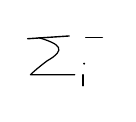
\begin{tikzpicture}[x=1pt,y=1pt,baseline=0pt,line cap=round,line join=round]
\path[use as bounding box] (0,-5) rectangle (29,19);
\node[anchor=base west,inner sep=0pt,outer sep=0pt] at (0,0) {$\phantom{\Sigma_i^-}$};
\draw[line width=.5pt] (0,15)--(15,16);
\draw[line width=.45pt] (4,15.4) .. controls (12,13) and (14,11) .. (7,7) .. controls (3,4) and (1,2) .. (1,2)--(17,2);
\draw[line width=.5pt] (20,2)--(20,-2);
\fill (20.4,6) circle (.4pt);
\draw[line width=.45pt] (21,15.5)--(27,15.5);
\end{tikzpicture}
% END C024-S05
tel que $\overline{U_{s_-}}\cap E_i\ne\varnothing$
% BEGIN GROUP A024-G22
% Owns the final parenthesis and comma only. Comma's left head-run retained.
\begin{tikzpicture}[x=.006cm,y=-.006cm,baseline={(1586,2263)}]
\path[use as bounding box] (1586,2158) rectangle (1635,2279);
\draw[gray,line width=.4pt] (1594,2162) .. controls (1604,2174) and (1602,2192) .. (1601,2204);
\draw[line width=.6pt] (1601,2205) .. controls (1599,2233) and (1594,2247) .. (1587,2249);
\draw[line width=.8pt] (1612,2251) -- (1626,2250);
\draw[line width=1.1pt] (1628,2244) .. controls (1632,2255) and (1619,2272) .. (1610,2277);
\end{tikzpicture}
% END GROUP A024-G22
% END UNIT P5
% BEGIN UNIT ARCHIVE
% archive sheet number: 23
% END UNIT ARCHIVE
